\documentclass[10pt,a4paper]{amsart}
\usepackage[margin=19mm]{geometry}
\usepackage{amsmath,amssymb,mathtools}
\usepackage[scr=rsfs,cal=euler]{mathalfa}
\usepackage{xfrac}
\usepackage[unicode,hidelinks,bookmarks=false]{hyperref}
\newcommand{\ie}{i.e.\ }
\newcommand{\cf}{cf.\ }
\newcommand{\resp}{respectively\ }
\newcommand{\Subsection}{\subsection}
\providecommand{\nobreakdash}{\nobreak\hbox{-}}
\setlength{\emergencystretch}{2em}
\multlinegap0pt
\usepackage{tikz}
\usepackage{float}
\usepackage{amssymb}
\usepackage{dsfont}
\usepackage{bm}
\usepackage[shortlabels]{enumitem}
\newtheorem{lemma}{Lemma}
\def\And{\mbox{\rm ~and~}}
\def\i{\mbox{\rm (\hspace{0.2mm}i\hspace{0.2mm})}\,}
\title{Polynomials Counting Group Colorings in Graphs}
\author{Houshan Fu}
\date{Source: arXiv:2409.12404v5 (CC BY 4.0)}
\begin{document}
\maketitle

\noindent\emph{Source and licence.} Polynomials Counting Group Colorings in Graphs. Version arXiv:2409.12404v5 (CC BY 4.0), distributed by arXiv under the Creative Commons Attribution 4.0 International licence, http://creativecommons.org/licenses/by/4.0/, as recorded in the arXiv licence metadata for this exact version and shown on the abstract page https://arxiv.org/abs/2409.12404v5. Full licence notice: \texttt{licenses/arxiv-2409.12404-CC-BY-4.0.txt}.\par\smallskip

\noindent\textit{Editorial scope.} Counted unit: the article's lemma No-Broken-Circuit (source0.tex lines 746--748). The article's complete original proof of it is delivered with it (source0.tex lines 749--827, one \texttt{proof} environment of 79 lines). No mathematics is written, repaired or re-derived: the statement and the proof are the article's own lines, in the article's own notation, and no retained line is substituted or re-flowed.  No further source-local context is needed: every cross-reference of every retained line resolves inside the two delivered spans.  Nothing was omitted from any retained span, so the package carries no omission record.  No retained line contains a citation, so the wrapper carries no bibliography and no bibliography entry.  The retained lines contain the article's own diagram code, which the wrapper typesets with the standard tikz packages; no image file is delivered and the package declares no asset dependency.  Editorial formatting only, in addition: an AMS \texttt{amsart} preamble that restates the article's own declarations and macros used by the retained lines, namely the environments \texttt{lemma} on separate counters, together with the standard packages those lines need.  The retained environments print in this document as Lemma 1 in order of appearance, whereas the article prints the same items with the numbering of its own full document.  The complete native source of the article as distributed in the arXiv e-print for this exact version is bundled unchanged as \texttt{sources/165480/source0.tex}.
\begin{lemma}\label{No-Broken-Circuit}
Let $\alpha$ be a $D$-admissible assigning of $G$ and $\prec$ a linear ordering on $E(G)$. Suppose $H$ is a subgraph of $G$ containing a broken $\alpha$-compatible cycle $B$ and $B=C-e_C$ for some $\alpha$-compatible cycle $C$ of $G$, where $e_C$ is the maximal member in $E(C)$ with respect to $\prec$. If $H$ is an $\alpha$-compatible subgraph of $G$ and $e_C\notin E(H)$, then $H+e_C$ is an $\alpha$-compatible subgraph.
\end{lemma}

\begin{proof}
Note that $C$ is a cycle in $H+e_C$, but not in $H$. If $H+e_C$ contains exactly one more cycle $C$ than $H$, there is nothing left to prove. Otherwise, $H+e_C$ contains at least one additional cycle compared to $H$, excluding the cycle $C$. Every such additional cycle, together with the cycle $C$, forms a theta-subgraph in $H+e_C$. Therefore, this case reduces to verifying that each such the theta-subgraph in $H+e_C$ is an $\alpha$-compatible subgraph of $G$. Without loss of generality, we only need to examine the following oriented theta-subgraph in $H+e_C$ with the orientation $D$, as shown in \autoref{Fg1}.
\begin{figure}[H]
\centering
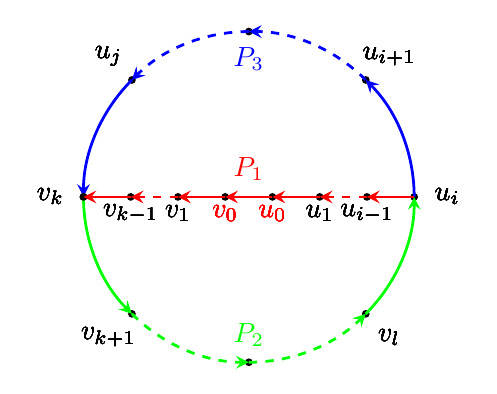
\begin{tikzpicture}[scale=0.7,line width=1pt]
\def\radius{3}
 \foreach \i in {1,...,8} {
        \pgfmathsetmacro{\angleA}{360/8 * (\i - 1)}
        \pgfmathsetmacro{\angleB}{360/8 * \i}
        \coordinate (P\i) at ({\radius * cos(\angleA)}, {\radius * sin(\angleA)});
        
        \fill (P\i) circle(2pt);
        \node at ({1.2*\radius * cos(360/8 * 0}, {1.2*\radius * sin(360/8 * 0)}) {$u_i$}; 
        \node at ({1.2*\radius * cos(360/8 * 1}, {1.2*\radius * sin(360/8 * 1)}) {$u_{i+1}$}; 
        \node at ({1.2*\radius * cos(360/8 * 3}, {1.2*\radius * sin(360/8 * 3)}) {$u_j$}; 
        \node at ({1.2*\radius * cos(360/8 * 4}, {1.2*\radius * sin(360/8 * 4)}) {$v_k$};  
        \node at ({1.2*\radius * cos(360/8 * 5}, {1.2*\radius * sin(360/8 * 5)}) {$v_{k+1}$};  
        \node at ({1.2*\radius * cos(360/8 * 7}, {1.2*\radius * sin(360/8 * 7)}) {$v_l$};  
    }
   \draw[-stealth,blue] (P1) arc[start angle=0,end angle=45,radius=\radius];     
    \draw[-stealth,dashed,blue] (P2) arc[start angle=45,end angle=90,radius=\radius];  
    \draw[-stealth,dashed,blue] (P3) arc[start angle=90,end angle=135,radius=\radius]; 
    \draw[-stealth,blue] (P4) arc[start angle=135,end angle=180,radius=\radius];  
    \draw[-stealth,green] (P5) arc[start angle=180,end angle=225,radius=\radius];  
    \draw[-stealth,dashed,green] (P6) arc[start angle=225,end angle=270,radius=\radius]; 
    \draw[-stealth,dashed,green] (P7) arc[start angle=270,end angle=315,radius=\radius]; 
    \draw[-stealth,green] (P8) arc[start angle=315,end angle=360,radius=\radius];  
\foreach \i in {1,...,7} {
        \pgfmathsetmacro{\fraction}{\i/7} 
        \coordinate (S\i) at ({(1-\fraction)*\radius*cos(0) + \fraction*\radius*cos(180)}, 
                              {(1-\fraction)*\radius*sin(0) + \fraction*\radius*sin(180)});
        \fill (S\i) circle(2pt);  
        \node at ({(1-1/7)*\radius*cos(0) + 1/7*\radius*cos(180)}, 
                  {(1-1/7)*\radius*sin(0) + 1/7*\radius*sin(180) - 0.3}) {$u_{i-1}$};  
        \node at ({(1-2/7)*\radius*cos(0) + 2/7*\radius*cos(180)}, 
                  {(1-2/5)*\radius*sin(0) + 2/5*\radius*sin(180) - 0.3}) {$u_1$}; 
        \node[red] at ({(1-3/7)*\radius*cos(0) + 3/7*\radius*cos(180)}, 
                  {(1-3/7)*\radius*sin(0) + 3/7*\radius*sin(180) - 0.3}) {$u_0$};  
        \node[red] at ({(1-4/7)*\radius*cos(0) + 4/7*\radius*cos(180)}, 
                  {(1-4/7)*\radius*sin(0) + 4/7*\radius*sin(180) - 0.3}) {$v_0$}; 
        \node at ({(1-5/7)*\radius*cos(0) + 5/7*\radius*cos(180)}, 
                  {(1-5/7)*\radius*sin(0) + 5/7*\radius*sin(180) - 0.3}) {$v_1$}; 
        \node at ({(1-6/7)*\radius*cos(0) + 6/7*\radius*cos(180)}, 
                  {(1-6/7)*\radius*sin(0) + 6/7*\radius*sin(180) - 0.3}) {$v_{k-1}$}; 
  }
\draw[-stealth,red] (P1) -- (S1);  
\draw[-stealth,dashed,red] (S1) -- (S2);
\draw[-stealth,red] (S2) -- (S3);
\draw[-stealth,red] (S3) -- (S4);
\draw[-stealth,red] (S4) -- (S5); 
\draw[-stealth,dashed,red] (S5) -- (S6); 
\draw[-stealth,red] (S6) -- (S7); 
\node[blue] at (0, \radius -0.5) {$P_3$}; 
\node[red] at (0, \radius -2.5) {$P_1$};    
\node[green] at (0, \radius -5.5) {$P_2$}; 
\end{tikzpicture}
\caption{The directed paths $P_1,P_2$ and $P_3$ toghter form an oriented theta-graph}\label{Fg1}
\end{figure}

More specifically, in \autoref{Fg1},  the edge $e_C=u_0v_0$; the cycle $C$, which is the union of the red directed path $P_1=(u_i,u_{i-1},\ldots,v_{k-1},v_k)$ and the green directed path $P_2=(v_k,v_{k+1},\ldots,v_l,u_i)$, and the cycle $C_1$, which is the union of  the red directed path $P_1$ and the blue directed path $P_3=(u_i,u_{i+1},\ldots,u_j,v_k)$, are in $H+e_C$ but not in $H$; the cycle $C_2$ is the common cycle of $H+e_C$ and $H$, formed by the union of both directed paths $P_2$ and $P_3$. Then, to complete our proof, it suffices to show $\alpha(C)=\alpha(C_1)=\alpha(C_2)=0$.

Since $\alpha$ is $D$-admissible, we may assume $\alpha=\alpha_{D,f}$ for some Abelian group $A$ and function $f:E(G)\to A$. Combining that $C$ and $H$ are $\alpha$-compatible subgraphs of $G$, this means 
\[
\alpha_{D,f}(C)=\alpha(C)=0\quad\And\quad\alpha_{D,f}(C_2)=\alpha(C_2)=0.
\]
This is further equivalent to satisfying the following equations
\[
\sum_{e\in E(C)}\eta_{D(C)}(e)f(e)=\sum_{e\in E(P_1)}\eta_{D(C)}(e)f(e)+\sum_{e\in E(P_2)}\eta_{D(C)}(e)f(e)=0
\]
and
\[
\sum_{e\in E(C_2)}\eta_{D(C_2)}(e)f(e)=\sum_{e\in E(P_2)}\eta_{D(C_2)}(e)f(e)+\sum_{e\in E(P_3)}\eta_{D(C_2)}(e)f(e)=0.
\]
Taking the clockwise as the reference direction for every cycle, then $\eta_{D(C_1)}(e)=-\eta_{D(C)}(e)$ for any edge $e\in E(P_1)$ and $\eta_{D(C_1)}(e)=\eta_{D(C_2)}(e)$ for any edge $e\in E(P_3)$. Thus, we deduce
\[
\sum_{e\in E(C_1)}\eta_{D(C_1)}(e)f(e)=\sum_{e\in E(P_1)}\eta_{D(C_1)}(e)f(e)+\sum_{e\in E(P_3)}\eta_{D(C_1)}(e)f(e)=0.
\]
This implies $\alpha(C_1)=\alpha_{D,f}(C_1)=0$. Therefore, $H+e_C$ is an $\alpha$-compatible subgraph of $G$.
\end{proof}

\end{document}
